\documentclass[a4paper]{article}

%Tutti gli usepackage vanno qui

\usepackage{geometry}
\usepackage[italian]{babel}
\usepackage[utf8]{inputenc}
\usepackage[T1]{fontenc}
\usepackage{tgschola}
%\usepackage{tgbonum}
\usepackage{tabularx}
\usepackage{longtable}
\usepackage{hyperref}
\usepackage{enumitem}
\usepackage[toc]{appendix}
\hypersetup{
	colorlinks=true,
	linkcolor=black,
	filecolor=magenta,      
	urlcolor=blue,
}
% Numerazione figure 
\let\counterwithout\relax
\let\counterwithin\relax
\usepackage{chngcntr}

\counterwithin{table}{subsection}
\counterwithin{figure}{subsection}

\usepackage[bottom]{footmisc}
\usepackage{fancyhdr}
\setcounter{secnumdepth}{4}
\usepackage{amsmath, amssymb}
\usepackage{array}
\usepackage{graphicx}

\usepackage{ifthen}

%\usepackage{float}
\usepackage{layouts}
\usepackage{url}
\usepackage{comment}
\usepackage{float}
\usepackage{eurosym}

\usepackage{lastpage}
\usepackage{layouts}
\usepackage{float}
\usepackage{eurosym}

%Comandi di impaginazione uguale per tutti i documenti
\pagestyle{fancy}
\lhead{
\includegraphics[scale=0.04]{../../../../latex/images/logoTWM.png}}
%Titolo del documento
\rhead{\doctitle{}}
%\rfoot{\thepage}
\cfoot{Pagina \thepage\ di \pageref{LastPage}}
\setlength{\headheight}{35pt}
\setcounter{tocdepth}{5}
\setcounter{secnumdepth}{5}
\renewcommand{\footrulewidth}{0.4pt}

% multirow per tabelle
\usepackage{multirow}

% Permette tabelle su più pagine
%\usepackage{longtable}


% colore di sfondo per le celle
\usepackage[table]{xcolor}

%COMANDI TABELLE
\newcommand{\rowcolorhead}{\rowcolor[HTML]{9b240a}} %intestazione 
% check for missing commands
\newcommand{\headertitle}[1]{\textbf{\color{white}#1}} %titolo colonna
\definecolor{pari}{HTML}{FFDBCB}
\definecolor{dispari}{HTML}{F1F7FD}

% comandi glossario
\newcommand{\glo}{$_{G}$}
\newcommand{\glosp}{$_{G}$ }


%label custom
\makeatletter
\newcommand{\uclabel}[2]{%
	\protected@write \@auxout {}{\string \newlabel {#1}{{#2}{\thepage}{#2}{#1}{}} }%
	\hypertarget{#1}{#2}
}
\makeatother

%riportare pezzi di codice
\definecolor{codegray}{gray}{0.9}
\newcommand{\code}[1]{\colorbox{codegray}{\texttt{#1}}}



% Configurazione della pagina iniziale
\newcommand{\doctitle}{Norme di Progetto}
\newcommand{\docdate}{ } % lasciare vuoto (uno carattere di spazio) per i documenti che non sono verbali, così non viene scritta la data
\newcommand{\rev}{3.0.1}
\newcommand{\stato}{Non Approvato}
\newcommand{\uso}{Interno}
\newcommand{\approv}{--De Renzis Simone}
\newcommand{\red}{Greggio Nicolò\\& Tessari Andrea}
\newcommand{\ver}{Zuccolo Giada\\& Crivellari Alberto}
\newcommand{\dest}{Three Way Milkshake\\ Prof. Vardanega Tullio\\ Prof.
 Cardin Riccardo}
\newcommand{\describedoc}{Questo documento contiene tutte le norme di progetto\textsubscript{G}, definite inizialmente o aggiunte in seguito, viene quindi aggiornato per incrementi successivi.}



 % modifica questo file
\makeindex

\usepackage{hyperref}
\usepackage{ulem}
\usepackage{listings}
\usepackage{float}

\begin{document}
	\thispagestyle{empty}
\begin{titlepage}
	\begin{center}
		
		
\includegraphics[scale = 0.17]{../../../../latex/images/logoTWM.png}\\[0.7cm]
		

		\noindent\rule{\textwidth}{1pt} \\[0.4cm]
		\Huge \textbf{\doctitle} \\[0.1cm]
		\ifthenelse{\equal{\docdate}{ }}{ }{ \huge \textbf{\docdate} \\[0.1cm] }
		
		\noindent\rule{\textwidth}{1pt}\\[0.7cm]
		
		\large \textbf{Three Way Milkshake - Progetto "PORTACS"} \\[0.4cm] 
                \texttt{threewaymilkshake@gmail.com} \\[0.4cm]
                
		
        
        
        \large

        \begin{tabular}{r|l}
                        \textbf{Versione} & \rev{} \\
                        \textbf{Stato} & \stato{} \\
                        \textbf{Uso} & \uso{} \\                         
                        \textbf{Approvazione} & \approv{} \\                      
                        \textbf{Redazione} & \red{} \\ 
                        \textbf{Verifica} &  \ver{} \\                         
                        \textbf{Destinatari} & \parbox[t]{5cm}{ \dest{} }
                \end{tabular} 
                \\[0.3cm]
                \large \textbf{Descrizione} \\ \describedoc{} 
               

	\end{center}
\end{titlepage}
	\pagebreak

	% Registro delle modifiche
	\section*{Registro delle modifiche}

\newcommand{\changelogTable}[1]{
	
	
	\renewcommand{\arraystretch}{1.5}
	\rowcolors{2}{pari}{dispari}
	\begin{longtable}{ 
			>{\centering}p{0.07\textwidth} 
			>{}p{0.21\textwidth}
			>{\centering}p{0.17\textwidth}
			>{\centering}p{0.13\textwidth} 
			>{\centering}p{0.17\textwidth} 
			>{\centering}p{0.13\textwidth} }
		\rowcolorhead
		\headertitle{Vers.} &
		\centering \headertitle{Descrizione} &	
		\headertitle{Redazione} &
		\headertitle{Data red.} & 
		\headertitle{Verifica} &
		\headertitle{Data ver.}
		\endfirsthead	
		\endhead
		
		#1
		
	\end{longtable}
	\vspace{-2em}
	
}


\newcommand{\approvingTable}[1]{ 
	
	
	\renewcommand{\arraystretch}{1.5}
	\rowcolors{2}{pari}{dispari}
	\begin{longtable}{ 
			>{\centering}p{0.07\textwidth} 
			>{\centering}p{0.415\textwidth}
			>{\centering}p{0.13\textwidth}
			>{\centering}p{0.322\textwidth}  }
		\rowcolorhead
		\headertitle{Vers.} &
		\centering \headertitle{Descrizione} &	
		\headertitle{Data appr.} &
		\headertitle{Approvazione}
		\endfirsthead	
		\endhead
		
		#1
		
	\end{longtable}
	\vspace{-2em}
	
}
	\changelogTable{
	3.5.0 & Incremento appendice \S\ A e B & Crivellari Alberto & 2021-04-26 & -- & --
	3.4.0 & Rimossa appendice \S\ D & Crivellari Alberto & 2021-04-01 & -- & --
	\tabularnewline
	3.3.0 & Modifica sezioni \S\ 2 e \S\ 3 & Crivellari Alberto & 2021-04-01 & -- & --
	\tabularnewline
	3.2.0 & Modifica appendice \S\ B & Zuccolo Giada & 2021-03-31 & -- & --
\tabularnewline
	3.1.0 & Aggiornamento appendice \S\ C & Crivellari Alberto & 2021-03-20 & -- & --
}

\approvingTable{
    3.0.0 & Approvazione del documento & 2021-03-08 & Zuccolo Giada
}

\changelogTable{
    2.1.0 & Aggiornamento sezioni \S\ 4 e 5 & Crivellari Alberto & 2021-03-08 & Chiarello Sofia & 2021-03-08
}

\approvingTable{
    2.0.0 & Approvazione del documento & 2021-02-22 & De Renzis Simone
}

\changelogTable{
1.3.0 & Completamento stesura appendice \S\ D e \S\ B & Crivellari Alberto & 2021-02-12 & Greggio Nicolò & 2021-02-19
\tabularnewline
1.2.1 & Completamento stesura sezione \S\ 2 e \S\ 3 & Chiarello Sofia & 2021-02-11 & Tessari Andrea & 2021-02-13
\tabularnewline
1.2.0 & Stesura sezione \S\ 3 e appendice \S\ C & Chiarello Sofia & 2021-02-09 & Tessari Andrea & 2021-02-12
\tabularnewline
1.1.0 & Stesura sezione \S\ 2 & Chiarello Sofia & 2021-02-08 & Tessari Andrea & 2021-02-13
}

\approvingTable{
	1.0.0 & Approvazione del documento & 2021-01-10 & De Renzis Simone
}

\changelogTable{
0.5.1 & Aggiunta tabelle a sezione \S 4 e \S5 & Crivellari Alberto & 2021-01-08 & Greggio Nicolò & 2021-01-10
\tabularnewline
0.5.0 & Redazione sezione \S 5 & Crivellari Alberto & 2020-12-07 & Greggio Nicolò & 2021-01-10
\tabularnewline
0.4.0 & Redazione sezione \S 4 & Crivellari Alberto & 2020-12-06 & Greggio Nicolò & 2021-01-10
\tabularnewline
0.3.2 & Modifiche sezione \S 1 & Crivellari Alberto & 2020-12-30 & Greggio Nicolò & 2021-01-10
\tabularnewline
0.3.1 & Tabelle sezione \S 3 & Crivellari Alberto & 2020-12-29 & Greggio Nicolò & 2021-01-10
\tabularnewline
0.3.0 & Redazione sezione \S 3 & Tessari Andrea & 2020-12-28 & Greggio Nicolò & 2021-01-10
\tabularnewline
0.2.1 & Tabelle sezione \S 2 & Crivellari Alberto & 2020-12-20 &  Greggio Nicolò & 2021-01-09
\tabularnewline
0.2.0 & Redazione sezione \S 2 & Crivellari Alberto & 2020-12-19 & Greggio Nicolò & 2021-01-09
\tabularnewline
0.1.1 & Modifiche sezione \S 1  & Crivellari Alberto & 2020-12-18 & Greggio Nicolò & 2021-01-09
\tabularnewline
0.1.0 & Redazione sezione \S 1 & Crivellari Alberto & 2020-12-16 & Greggio Nicolò & 2021-01-09
\tabularnewline
0.0.1 & Strutturazione del documento & Tessari Andrea & 2020-12-15 & Greggio Nicolò & 2021-01-09
}


 % modifica questo file
	\pagebreak

	% indice
	{
    	\hypersetup{linkcolor=black}
    	\tableofcontents
    	\pagebreak

        % indice delle figure, non ci sono figure
        \listoffigures
        \pagebreak

        % indice delle tabelle
        \listoftables
        \pagebreak
	}


	% contenuto del documento, ogni sezione in un file
	\section{Introduzione}
\subsection{Scopo del documento}
    Questo documento ha lo scopo di fissare e definire tutte le regole, convenzioni e buone pratiche utili a formare un way of working condiviso alla base da tutti i componenti del gruppo per assicurare una collaborazione efficiente ed efficace. Si discuteranno inoltre i vari strumenti che verranno adottati per facilitare lo sviluppo del progetto\textsubscript{G} e per promuovere un'organizzazione adeguata.
    Si ritiene inoltre che la definizione ed il mantenimento per incremento di un documento condiviso all'interno del gruppo di lavoro, che definisca e raccolga quanto descritto in maniera formale e centralizzata, possa favorire, in un contesto dove i membri possano variare, l'inserimento di nuovi componenti facilitandone l'ambientamento. Pur non essendo questo il contesto di lavoro attuale, è comunque una buona pratica da sperimentare e consolidare.

\subsection{Scopo del prodotto}
Il capitolato\textsubscript{G} C5 propone un progetto\textsubscript{G} in cui viene richiesto lo sviluppo di un software per il monitoraggio in tempo reale di unità che si muovono in uno spazio definito. All'interno di questo spazio, creato dall'utente per riprodurre le caratteristiche di un ambiente reale, le unità dovranno essere in grado di circolare in autonomia, o sotto il controllo dell'utente, per raggiungere dei punti di interesse posti nella mappa.  La circolazione è sottoposta a vincoli di viabilità e ad ostacoli propri della topologia dell'ambiente, deve evitare le collisioni con le altre unità e prevedere la gestione di situazioni critiche nel traffico.

\subsection{Termini, abbreviazioni ed altri documenti}
    Tutti i termini che necessitano di una spiegazione, per fornire un'adeguata comprensione, o perché possono causare ambiguità nel contesto, sono definiti nel glossario. A dispetto di tutti gli altri documenti presenti, il glossario è sotto la veste di una pagina web, più nello specifico in una wiki\textsubscript{G} di GitHub, accessibile a \href{https://github.com/Three-Way-Milkshake/docs/wiki/Glossario}{questo indirizzo}, con vocaboli suddivisi tra "Acronimi" e "Termini", disposti in ordine alfabetico al fine di facilitare la navigazione. All'interno dei documenti le voci di glossario saranno seguite da una G pedice mentre gli acronimi da una A (e.g.: voce di glossario\textsubscript{G} ; acronimo\textsubscript{A}).
    Inoltre quando si farà riferimento ad un altro documento o al documento stesso, il nome di questo sarà in maiuscoletto (e.g.: \textsc{esempio nome documento}).

\subsection{Riferimenti}
\label{ref}
    \subsubsection{Riferimenti Normativi}
        \begin{itemize}
            \item Standard ISO 12207:\\ \url{https://www.math.unipd.it/~tullio/IS-1/2009/Approfondimenti/ISO_12207-1995.pdf};
            \item Standard UML\textsubscript{A} 2.0:\\\url{https://www.omg.org/spec/UML/2.0/Superstructure/PDF};
            \item Diagrammi dei casi d'uso\textsubscript{G}:\\\url{https://www.math.unipd.it/~rcardin/swea/2021/Diagrammi\%20Use\%20Case_4x4.pdf};
            \item Diagrammi delle classi:\\\url{https://www.math.unipd.it/~rcardin/swea/2021/Diagrammi\%20delle\%20Classi_4x4.pdf};
            \item Diagrammi dei package:\\\url{https://www.math.unipd.it/~rcardin/swea/2021/Diagrammi\%20dei\%20Package_4x4.pdf};
            \item Diagrammi di attività\textsubscript{G}:\\\url{https://www.math.unipd.it/~rcardin/swea/2021/Diagrammi\%20di\%20Attivit\%c3\%a0_4x4.pdf};
            \item Diagrammi di sequenza:\\\url{https://www.math.unipd.it/~rcardin/swea/2021/Diagrammi\%20di\%20Sequenza_4x4.pdf};
            \item Standard ISO 8601:\\\url{https://www.iso.org/iso-8601-date-and-time-format.html}.
        \end{itemize}

    \subsubsection{Riferimenti Informativi}
        \begin{itemize}
        	\item \textsc{\href{https://github.com/Three-Way-Milkshake/docs/wiki/Glossario}{Glossario}}:\\per la definizione dei termini (pedice G) e degli acronimi (pedice A) evidenziati nel documento;
            \item \url{https://www.math.unipd.it/~tullio/IS-1/2020/Dispense/L03.pdf}
            \item \url{https://www.math.unipd.it/~tullio/IS-1/2020/Dispense/L06.pdf}
            \item \url{https://www.math.unipd.it/~tullio/IS-1/2020/Dispense/FC2.pdf}
            \item \url{https://www.math.unipd.it/~rcardin/swea/2021/SOLID\%20Principles\%20of\%20Object-Oriented\%20Design_4x4.pdf}
            \item \url{https://www.math.unipd.it/~tullio/IS-1/2020/Dispense/L09.pdf}
            \item \url{https://docs.github.com/en/free-pro-team@latest/actions}
            \item \url{https://www.latex-project.org/}
            \item \url{http://www.texstudio.org/}
            \item \url{https://www.xm1math.net/texmaker/}
            \item \url{https://www.atlassian.com/git/tutorials/comparing-workflows/gitflow-workflow}
            \item \url{https://github.com/about}
            \item \url{https://www.atlassian.com/software/jira}
            \item \url{https://www.atlassian.com/}
            \item \url{https://meet.google.com/}
            \item \url{https://slack.com/intl/en-it/about}
            \item \url{https://telegram.org/}
            \item \url{https://workspace.google.com/products/chat/}
        \end{itemize}

\pagebreak

	\pagebreak

	\section{Visione generale delle strategie di gestione della qualità}
In questa sezione vengono illustrati gli obiettivi fissati dal gruppo per garantire la qualità di processo e di prodotto nella realizzazione del progetto\textsubscript{G}.
Al fine di monitorare costantemente lo stato e il raggiungimento degli obiettivi, sono stati adottati standard e metriche adeguate, le quali verranno illustrate in dettaglio nelle sezioni successive.
Sia gli obiettivi che le metriche sono identificati univocamente da un codice alfanumerico in modo da renderli facilmente tracciabili e quindi controllabili costantemente.

\subsection{Qualità di processo}
Vista l’importanza della qualità di processo per ottenere un prodotto valido nei tempi prestabili si è deciso di usare gli standard ISO/IEC 12207 e ISO/IEC 25010:2011, semplificandoli e riadattandoli in base alle esigenze. Viene riportata una descrizione di tali standard nell'appendice \S\ D.

\subsection{Qualità del prodotto}
Per valutare la qualità del prodotto, il gruppo Three Way Milkshake ha deciso di avvalersi dello standard ISO/IEC 9126 descritto nell'appendice \S\ D. Tale standard definisce i criteri di applicazione delle metriche descritte nella sezione \S\ 2.4, utilizzate per valutare il livello del raggiungimento degli obiettivi descritti nella tabella 2.3.1.
I prodotti realizzati sono:
\begin{itemize}
    \item \textbf{documentazione}: deve essere leggibile e priva di errori ortografici, sintattici, logici e semantici;
    \item \textbf{software}: 
    \begin{itemize}
        \item deve possedere tutti i requisiti obbligatori descritti nell'\textsc{Analisi dei Requisiti};
        \item deve essere leggibile, comprensibile e mantenibile;
        \item deve essere ampiamente testato e robusto.
    \end{itemize}
\end{itemize}

\subsection{Tabella Obiettivi}
Viene presentata in seguito la tabella degli obiettivi di qualità prefissati e le relative metriche di misura.



\renewcommand{\arraystretch}{1.5}
\rowcolors{2}{pari}{dispari}
\begin{longtable}{ 
		>{}p{0.1\textwidth} 
		>{}p{0.18\textwidth}
        >{}p{0.35\textwidth}
        >{\centering}p{0.30\textwidth} }
        
	\rowcolorhead
	\centering \headertitle{Codice} &
	\centering \headertitle{Nome} &	
    \centering \headertitle{Descrizione} &
    \centering \headertitle{Metriche}	
	\endfirsthead	
    \endhead
    
        01 & Miglioramento continuo & Capacità del processo di misurare e migliorare le proprie capacità & 
                         \textbf{REI}: Rapporto riunioni Esterne e Interne \newline
                         \textbf{RRL}: Rapporto tempo Riunioni e Lavoro individuale \newline
                         \textbf{RTEI}: Rapporto Tempo Effettivo totale e Individuale \newline
                         \textbf{DLE}: Distribuzione Lavoro Effettivo \newline
                         \textbf{RTPI}: Rapporto Tempo Preventivato totale e Individuale \newline
                         \textbf{DLP}: Distribuzione Lavoro Preventivato \newline 
                         \textbf{DTEP}: Differenza Tempo Effettivo e Preventivato \newline 
                         \textbf{PDTT}: Percentuale Discostamento Totale (in Tempo) \newline 
                         \textbf{PDTR}: Percentuale Discostamento Totale (in Ritardo) \newline 
                         \textbf{PDTA}: Percentuale Discostamento Totale (in Anticipo) \newline 
                         \textbf{PDDWT}: Percentuale Discostamento DoneWorking (in Tempo) \newline 
                         \textbf{PDDWR}: Percentuale Discostamento DoneWorking (in Ritardo) \newline 
                         \textbf{PDDWA}: Percentuale Discostamento DoneWorking (in Anticipo) \newline 
                         \textbf{PDDVT}: Percentuale Discostamento DoneVerifying (in Tempo) \newline
                         \textbf{PDDVR}: Percentuale Discostamento DoneVerifying (in Ritardo) \newline
                         \textbf{PDDVA}: Percentuale Discostamento DoneVerifying (in Anticipo) \newline
                         \textbf{SRI}: Scarto Riun. Interne \newline 
                         \textbf{SRE}: Scarto Riun. Esterne 
                         \tabularnewline

        02 & Leggibilità dei documentazione & I documenti devono essere leggibili e comprensibili da persone con licenza di scuola media/superiore & \textbf{IG}: Indice di Gulpease \tabularnewline

        03 & Implementazione Requisiti Obbligatori & Devono venire implementati tutti i requisiti obbligatori descritti dall'\textsc{Analisi dei Requisiti} & \textbf{PROS}: Requisiti Obbligatori Soddisfatti \tabularnewline

        04 & Manutenzione e comprensione del codice & Il codice deve essere quanto più comprensibile e mantenibile & \textbf{CBO}: Coupling Between Objects \newline \textbf{DEP}: DEPth of hierarchies \newline \textbf{LEV}: LEVel of nesting \newline \textbf{PAR}: PARametri per metodo \newline \textbf{ATT}: ATTributi per classe \newline \textbf{MET}: METodi per classe \newline\textbf{RCC}: Rapporto Codice Commenti \newline\textbf{{CCL}}: Complessità CicLomatica \tabularnewline

        05 & Copertura del codice & Il codice dovrà essere testato in ogni sua parte per garantire le funzionalità previste dai requisiti & \textbf{CC}: Code Coverage \tabularnewline

        06 & Superamento test & La Percentuale di superamento dei test dovrà essere $\geq 80$ del totale & \textbf{PST}: Percentuale Superamento Test \tabularnewline

        07 & Conformità & Il prodotto dovrà essere conforme ai requisiti, implementando le funzionalità richieste & \textbf{CS}: Completezza del Software \tabularnewline

        08 & Robustezza & Il prodotto dovrà far fronte a situazioni anomale gestendole senza arrestare la sua esecuzione & \textbf{A}: Affidabilità del software \tabularnewline

        09 & Usabilità & Il prodotto dovrà essere il più semplice possibile da utilizzare & \textbf{C}: numero di tocchi/Click necessari \newline \textbf{S}: numero di Secondi necessari\tabularnewline
        \caption{Tabella Obiettivi}
    \end{longtable}



\subsection{Metriche}
Per raggiungere gli obiettivi di qualità è necessario che il processo di verifica produca dei risultati quantificabili, così da poterli confrontare con gli obiettivi fissati a priori. Per questo vengono prefissate delle metriche e dei valori di sufficienza minimi necessari, i quali serviranno a controllare che i livelli qualitativi di processo e di prodotto siano in linea con gli obiettivi prefissati.\\La seguente tabella riporta le metriche utilizzate, le rispettive soglie di valori preferibili e accetabili e i relativi obiettivi, così da poter monitorare e controllare gli obiettivi raggiunti e gli eventuali progressi.

%sistemare
\renewcommand{\arraystretch}{1.5}
\rowcolors{2}{pari}{dispari}
\begin{longtable}{ 
		>{\centering}p{0.1\textwidth} 
		>{}p{0.18\textwidth}
        >{\centering}p{0.20\textwidth}
        >{\centering}p{0.20\textwidth}
        >{}p{0.12\textwidth} }
        
	\rowcolorhead
	\centering \headertitle{Codice} &
	\centering \headertitle{Nome} &	
    \centering \headertitle{Valori Preferibili} &
    \centering \headertitle{Valori Accettabili}	&
    \centering \headertitle{Obiettivi}	
	\endfirsthead	
    \endhead

            REI & Rapporto riunioni Esterne e Interne & $0.4 \leq REI \leq 0.5$ & $0.3 \leq REI \leq 0.5$ & 01\\

            RRL & Rapporto tempo Riunioni e Lavoro individuale & $0.08 \leq RRL \leq 0.12$ & $0.08 \leq RRL \leq 0.4$ & 01 \\

            RTEI & Rapporto Tempo Effettivo totale e Individuale & $0.17$ & $0.15 \leq RTEI \leq 0.19$ & 01 \\

            DLE & Distribuzione Lavoro Effettivo & $0 \leq DLE \leq 600$ & $0 \leq DLE \leq 900$ & 01 \\

            RTPI & Rapporto Tempo Preventivato totale e Individuale & $0.17$ & $0.15 \leq RTPI \leq 0.19$ & 01 \\

            DLP & Distribuzione Lavoro Preventivato & $0 \leq DLP \leq 600$ & $0 \leq DLP \leq 900$ & 01 \\

            DTEP & Differenza Tempo Effettivo e Preventivato & $0$ & $-600 \leq DTEP \leq 600$ & 01 \\

            PDTT & Percentuale Discostamento Totale (in Tempo) & $1$ & $PDTT \geq 0.4$ & 01 \\

            PDTR & Percentuale Discostamento Totale (in Ritardo) & $0$ & $PDTR \leq 0.3$ & 01 \\   
            
            PDTA & Percentuale Discostamento Totale (in Anticipo) & $0$ & $PDTA \leq 0.3$ & 01 \\

            PDDWT & Percentuale Discostamento DoneWorking (in Tempo) & $1$ & $PDDWT \geq 0.4$ & 01 \\

            PDDWR & Percentuale Discostamento DoneWorking (in Ritardo) & $0$ & $PDDWR \leq 0.3$ & 01 \\   
            
            PDDWA & Percentuale Discostamento DoneWorking (in Anticipo) & $0$ & $PDDWA \leq 0.3$ & 01 \\

            PDDVT & Percentuale Discostamento DoneVerifying (in Tempo) & $1$ & $PDDVT \geq 0.4$ & 01 \\

            PDDVR & Percentuale Discostamento DoneVerifying (in Ritardo) & $0$ & $PDDVR \leq 0.3$ & 01 \\   
            
            PDDVA & Percentuale Discostamento DoneVerifying (in Anticipo) & $0$ & $PDDVA \leq 0.3$ & 01 \\

            SRI & Scarto Riunioni Interne & 0 & $-90 \leq SRI \leq 90$ & 01 \\

            SRE & Scarto Riunioni Esterne &  0 & $-90 \leq SRE \leq 90$ & 01 \\

            IG & Indice di Gulpease & $70 \leq IG \leq 100$ & $50 \leq IG \leq 100$ & 02 \\

            PROS & Requisiti Obbligatori Soddisfatti & 100\% & 100\% & 03 \\

            CBO & Coupling Between Objects & $0\leq CBO \leq 1$ & $0\leq CBO \leq 6$ & 04 \\

            DEP & DEPth of hierarchies & $DEP \leq 2$ & $DEP \leq 3$ & 04 \\

            LEV & LEVel of nesting & $1\leq LEV \leq 3$ & $1\leq LEV \leq 6$ & 04 \\

            PAR & PARametri per metodo & $PAR \leq 4$ & $PAR \leq 6$ & 04 \\

            ATT & ATTributi per classe & $0 \leq ATT \leq 8$ & $0 \leq ATT \leq 15$ & 04 \\

            MET & METodi per classe & $0 \leq MET \leq 5$ & $0 \leq MET \leq 15$ & 04 \\

            RCC & Rapporto Codice Commenti & $RCC \geq 0.4$ & $RCC \geq 0.2$  & 04 \\

            CCL & Complessità CicLomatica & $CCL \leq 10 $ & $CCL \leq 20 $& 04 \\

            CC & Code Coverage & $CC\leq 70\%$ & $CC\leq 50\%$ & 05 \\

            PST & Percentuale Superamento Test & 100\% & 85\% & 06 \\

            DEP & DEepth of hierarchies & $DEP \leq 2$ & $DEP \leq 3$ & 05 \\

            LEV & Level of nesting & $1\leq LEV \leq 3$ & $1\leq LEV \leq 6$ & 05 \\

            PAR & Parametri per metodo & $PAR \leq 4$ & $PAR \leq 6$ & 05 \\

            ATT & Attributi per classe & $0 \leq ATT \leq 8$ & $0 \leq ATT \leq 15$ & 05 \\

            MET & Metodi per classe & $0 \leq MET \leq 5$ & $0 \leq MET \leq 15$ & 05 \\

            CS & Completezza del Software & $CS=1$ & $CS=1$ & 07 \\

            A & Affidabilità del software & $A=0$ & $A < 0.15$ & 08 \\

           C & numero di tocchi/Click necessari & $C<4$ & $C<6$& 09 \\

           S & numero di Secondi necessari & $S<15$ & $S<40$ & 09 \\

           
           \caption{Tabella delle Metriche}
        \end{longtable}



	\pagebreak

	\section{Gestione amministrativa}
\subsection{Misure e metriche in dettaglio}
In questa sezione vengono descritte in dettaglio le varie metriche utilizzate, con una breve descrizione e la modalità di calcolo. 
Le soglie di accettabilità sono riportate nella tabella 2.4.1 "Tabella delle Metriche", valori inferiori ai limiti accettabili sono considerati negativi e il prodotto o processo dovrà essere sottoposto ad ulteriori indagini e verifiche.
\subsection{Metriche per i processi}
\subsubsection{Scarto riunioni (SR)}
Viene utilizzata alla fine di ogni periodo per monitorare e valutare una ripianificazione delle riunioni. Viene rappresentato tramite la differenza tra il tempo preventivato della durata di una riunione e la sua durata effettiva. Sono identificati tre sottometriche in base al tipo di riunione:
\begin{itemize}
    \item scarto riunioni;
    \item scarto riunioni interne;
    \item scarto riunioni esterne.
\end{itemize}

\subsubsection{Totale riunioni (TR)}
Viene tenuto traccia il numero totale di riunioni effettuate.
\subsubsection{Totale riunioni interne (TRI)}
Viene tenuto traccia il numero totale di riunioni interne effettuate.
\subsubsection{Totale riunioni esterne (TRE)}
Viene tenuto traccia il numero totale di riunioni esterne con il proponente effettuate.

\subsubsection{Scarto ticket (ST)}
Anch'esso utilizzato alla fine di ogni periodo per monitorare e valutare una ripianificazione sul tempo assegnato ad ogni ticket per completarlo. 
\[
    (tempo preventivato completamento ticket)-(tempo effettivo completamento ticket)
\]

\subsubsection{Differenza ToVerify (DV)}
Metrica utilizzata per monitorare il tempo impiegato per eseguire un ticket, ossia da passare dallo stato \textit{To Do} a \textit{To Verify}. Viene calcolato ..

\subsubsection{Differenza Done Verify (DD)}
Metrica utilizzata per monitorare il tempo impiegato per eseguire un ticket, ossia da passare dallo stato \textit{To Verify} a \textit{Done Verify}. Viene calcolato ..

\subsubsection{Uniformità del lavoro nel tempo (UL)}
Per ogni periodo, vengono contati il numero di ticket passati a \textit{To Verify} e quelli passati a \textit{Done Verify}.

\subsubsection{Budget At Completion (BAC)}
Indica il budget totale allocato per il progetto.

\subsubsection{Earned Value (EV)}
Indica la quantità di guadagno ottenuta dal lavoro effettuato fino al momento di calcolo.
\[
    (preventivo)*(\%\_lavoro\_completato)
\]

\subsubsection{Planned Value (PV)}
Indica la quantità di guadagno stimata sul lavoro pianificato al momento del calcolo.
\[
    (preventivo)*(\%\_lavoro\_pianificato)
\]

\subsubsection{Schedule Variance (SV)}
Indica l'anticipo o il ritardo del lavoro effettuato rispetto alla pianificazione.
\[
    EV - PV
\]

\subsubsection{Actual Cost (AC)}
I costi sostenuti fino al momento del calcolo.

\subsubsection{Cost Variance (CV)}
La differenza tra il costo del lavoro ad ora effettuato e quello preventivato.

\[
    EV-AC
\]

\subsection{Metriche per la documentazione}

\subsection{Indice di Gulpease (IG)}
Indica la leggibilità di un testo, tarato sulla lingua italiana. Differentemente da indici di lingua straniera, ha il vantaggio di controllare la lunghezza delle parole anzichè il numero di sillabe per parola, semplificandone il calcolo automatico. 
Nel calcolo vengono ignorati frontespizio, registro modifiche, elenco figure, elenco ta-belle e figure e tabelle; in modo da poter valutare appieno la leggibilità del contenutotestuale dei documenti.
Il valore risultante è compreso tra 0 e 100, dove un indice più alto corrisponde ad un indice di leggibilità più semplice.
Le soglie dei valori dell’indice di leggibilità Gulpease sono:
\begin{itemize}
    \item inferiore a 80, il documento `e difficile da leggere per chi ha la licenza elementare;
    \item inferiore a 60, il documento `e difficile da leggere per chi possiede la licenza media;
    \item inferiore a 40, il documento `e difficile da leggere per chi ha un diploma superiore.
\end{itemize}
\[
    89+ \frac{300\cdot (num\_frasi) - 10\cdot (num\_lettere)}{num\_parole}
\]

\subsection{Metriche per il software}
Questa sezione contiene le metriche che si cercherà di applicare al software prodotto. A causa dell’inesperienza del gruppo, tali valori sono una dichiarazione di intenti per la qualità del software e potrebbero essere rivisti con le successive revisioni.

\subsubsection{Percentuale Requisiti Obbligatori Soddisfatti (PROS)}
Indica la quantità di requisiti obbligatori soddisfatti rispetto al totale.
\[\frac{requisiti\_obbligatori\_soddisfatti}{requisiti\_obbligatori\_totali}\]

\subsubsection{Coupling Between Objects (CBO)}
Indica l'accoppiamento tra classi e oggetti; due classi si dicono accoppiate se una utilizza metodi o variabili dell'altra.

\subsubsection{DEPth of hierarchies(DEP)}
Indica la profondità delle gerarchie nel codice sviluppato.

\subsubsection{LEVel of nesting (LEV)}
Indica il livello di annidamento nei vari metodi presenti nel codice prodotto.
\textbf{Profondità della gerarchia dei collegamenti (P)}\\
Viene specificata la profondità gerarchica massima dei collegamenti e delle funzionalità presenti all'interno del software.
\begin{itemize}
	\item \textbf{misurazione:} profondità gerarchica massima dei collegamenti e delle funzionalità presenti all'interno del software;
	\item \textbf{valore preferibile:} $P < 4$;
	\item \textbf{valore accettabile:} $P < 6$.
\end{itemize}

\subsubsection{PARametri per metodo (PAR)}
Indica il numero di parametri presenti nei metodi sviluppati nel codice.

\subsubsection{Rapporto Codice Commenti (RCC)}
Indica il rapporto tra le linee di codice e le linee di commento all'interno del file.
\[\frac{linee\_codice}{linee\_commento}\]

\subsubsection{Code Coverage (CC)}
Indica la quantità di codice che viene effettivamente eseguito durante i test; aiuta a valutare la completezza di questi.
\[\frac{linee\_codice\_verificate}{linee\_codice\_totali}\]

\subsubsection{Completezza del Software(Cs)}
Viene specificata la completezza del software.
\[C = (1- \frac{funzionalita\_non\_implementate }{funzionalita\_implementate})\]

\subsubsection{Affidabilità del Software (A)}
Viene specificata l'abilità del software di resistere a malfunzionamenti.
\[A = \frac{numero\_di\_errori}{numero\_di\_test\_eseguiti}\]

\subsubsection{Numero di tocchi/click necessari (C)}
Viene specificata la facilità con cui l'utente riesce a raggiungere ciò che vuole attraverso il conteggio del numero di tocchi o click necessari al suo raggiungimento.\\
Si considera la capacità dell'operatore di visualizzare la propria lista delle task.

\subsubsection{Numero di secondi necessari (S)}
Viene specificata la facilità con cui l'utente riesce a raggiungere ciò che vuole attraverso il conteggio dei secondi necessari al suo raggiungimento.\\
Si considera la capacità dell'operatore di visualizzare la propria lista delle task.

\subsubsection{Leggibilità del Software (L)}
\[\frac{numero\_di\_linee\_di\_codice\_commentate}{numero\_di\_linee\_di\_codice}\]

\subsection{Comunicazione e risoluzione delle anomalie}

Questa attività è finalizzata alla tempestiva individuazione e risoluzione delle anomalie, ovvero le deviazioni del piano prefissato. Rappresentano un'anomalia:
\begin{itemize}
    \item violazioni delle norme tipografiche prefissate;
    \item presenza di contenuti non inerenti con l'argomento trattato;
    \item mancato rispetto dei valori contenuti in questo documento;
    \item incongruenze tra il prodotto e le funzionalità descritte nell'\textsc{Analisi dei Requisiti};
\end{itemize}
Nel caso venga individuata una nuova anomalia, deve essere segnalata tempestivamente, nella modalità descritta nelle \textsc{Norme di Progetto}. In questo modo il Responsabile sarà informato dell'anomalia e sarà possibile gestirla in modo corretto.

	\pagebreak
	\appendix
	\section{Test}

\subsection{Specifica dei test}

Per garantire la qualità del prodotto, \textit{Three Way Milkshake} adotta il Modello a V per verificare tramite test ogni passo della produzione software.\\Qui vedremo un immagine rappresentativa del \gls{vmodel}\textsubscript{G} (o V-Model), quest'ultimo si puo' schematizzare posizionando il tempo nell'asse delle ascisse e il livello di astrazione nell'asse delle ordinate.\\Il modello idealmente si divide in 2 rami.\\Il ramo sinistro contiene le fasi di progettazione e ideazione; il ramo destro contiene le fasi di testing e integrazione.
\begin{figure}[h!]
	\centering
	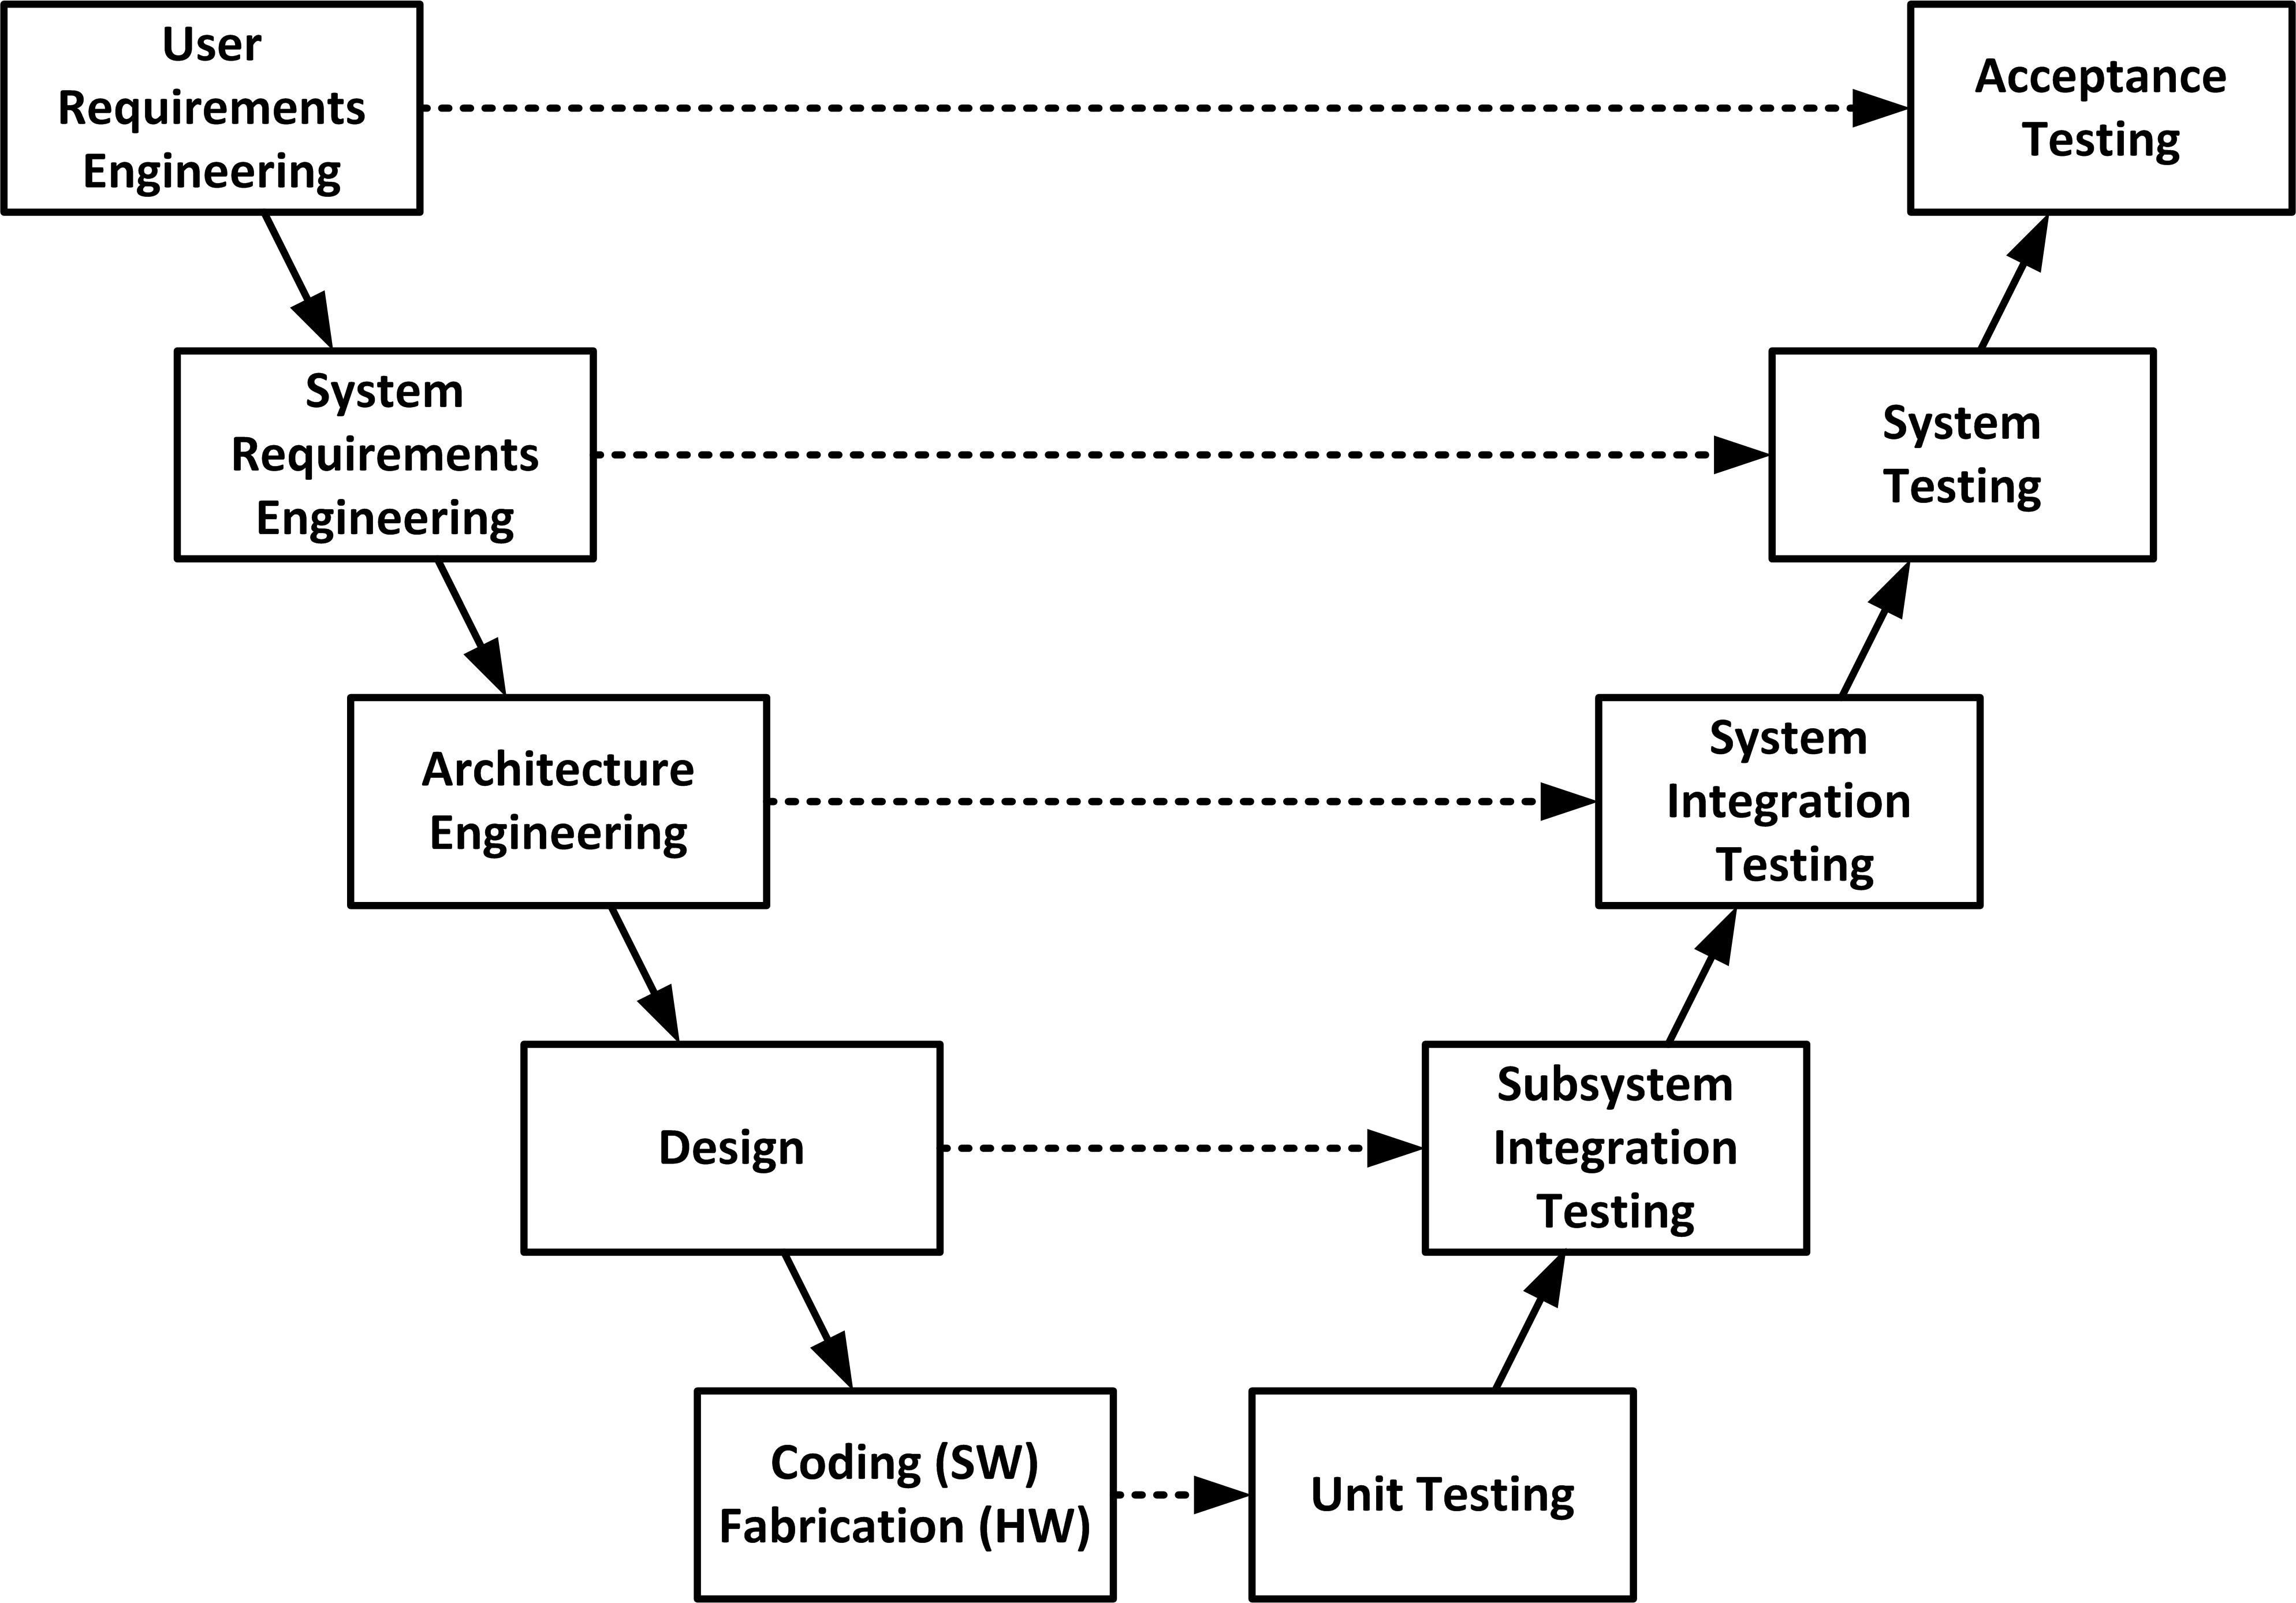
\includegraphics[scale=0.6]{res/images/v_model.jpg}
	\caption{Figura esplicativa del \gls{vmodel}\textsubscript{G}}
\end{figure}

\subsection{Test di accettazione}

\subsection{Test di sistema}

\subsection{Test di integrazione}

\subsection{Test d'unità}

\subsection{Resoconto attività di verifica}
\subsubsection{Esiti dell'indice di Gulpease}

	\pagebreak

	\section{Resoconto \gls{attivita}\textsubscript{G} di verifica}
\subsection{Esiti dell'indice di Gulpease}
% COMPILARE VALORI GULPEASE e METTERE DATE VERBALI
\begin{table}[H]
	\begin{center}
		\caption{Tabella dei valori Gulpease}
		\begin{tabular}{ccc}
			\rowcolorhead
			\headertitle{Nome Documento} & \headertitle{Valore Gulpease} & \headertitle{Esito}\\

			\textsc{Analisi dei Requisiti} v1.0.0 & & Superato\\
			\textsc{Glossario} v1.0.0 & & Superato\\
			\textsc{Norme di Progetto} v1.0.0 & & Superato\\
			\textsc{Piano di Qualifica} v1.0.0 & & Superato\\
			\textsc{Piano di Progetto} v1.0.0 & & Superato\\
			\textsc{Verbale Esterno 1} & & Superato\\
			\textsc{Verbale Esterno 2} & & Superato\\
			\textsc{Verbale Interno 1} & & Superato\\
			\textsc{Verbale Interno 2} & & Superato\\
			\textsc{Verbale Interno 3} & & Superato\\
			\textsc{Verbale Interno 4} & & Superato\\
			\textsc{Verbale Interno 2021-01-04} & & Superato\\

		\end{tabular}

	\end{center}
\end{table}
	\pagebreak

	\section{Valutazioni per il miglioramento}
L'obiettivo di questa sezione è la valutazione atta al miglioramento dell'intero processo produttivo legato al progetto\textsubscript{G} in corso. Risulta necessario trovare un modo per affrontare i problemi che possono sorgere durante il lavoro, così da poter proporre soluzioni efficienti per la loro risoluzione. E` inoltre necessario tenere traccia dei problemi riscontrati e delle loro soluzioni, così che essi non vengano ripetuti.
Più in dettaglio si valuteranno i problemi legati a:
\begin{itemize}
    \item organizzazione: qualsiasi problema inerente all'organizzazione e alla collaborazione del gruppo;
    \item ruoli: qualsiasi problema legato allo svolgimento di un ruolo;
    \item strumenti: qualsiasi problema riscontrato nell'utilizzo di determinati strumenti.
\end{itemize}

Una difficoltà rilevante in queste valutazioni è il fatto che sono gestite dal gruppo stesso, quindi si tratta di un'autovalutazione. Ogni singolo membro deve esternare i propri problemi individuali e quelli di gruppo per permettere una celere risoluzione e favorire un lavoro più efficiente.
Tale sezione mira quindi a migliorare costantemente la qualità di prodotto, infatti verrà aggiornata durante l'intero periodo\textsubscript{G} di progetto\textsubscript{G} man mano che si verificheranno problemi.
Vi è inoltre una sezione riguardante i  rischi all'interno del \textsc{Piano di Progetto} con la loro descrizione e relativa soluzione a completamento di questa parte sui possibili problemi.
\subsection{Valutazioni sull'organizzazione}
\renewcommand{\arraystretch}{1.5}
\rowcolors{2}{pari}{dispari}
\begin{longtable}{
    >{}p{0.5\textwidth}
        >{}p{0.5\textwidth}
}
\rowcolorhead
\centering \headertitle{Problema} &
\centering \headertitle{Soluzione}
\endfirsthead
\endhead
Durante i primi periodi si ha avuto difficoltà a comunicare con tutti i membri del gruppo, avendo difficoltà a organizzare gli incontri e a ricevere risposta per domande o chiarificazioni sul proprio lavoro & Si è deciso di utilizzare come sistema di comunicazione ufficiale Slack così, oltre ad avere diversi topic di conversazione, si ha un promemoria automatico per l'avviso di nuove riunioni \\

Difficoltà nel rispettare le scadenze dei lavori assegnati; probabile causa la scarsa esperienza di pianificazione e quindi erronea stima del tempo impiegato per un determinato lavoro & Come soluzione si è deciso di rispettare di più le scadenze, lavorando più del periodo\textsubscript{G} passato e di stimare le scadenze con più cura. \\
\caption{Tabella Problemi di organizzazione}
    \end{longtable}

\subsection{Valutazioni sui ruoli}

\subsubsection{Analista}
\renewcommand{\arraystretch}{1.5}
\rowcolors{2}{pari}{dispari}
\begin{longtable}{
    >{}p{0.5\textwidth}
        >{}p{0.5\textwidth}
}
\rowcolorhead
\centering \headertitle{Problema} &
\centering \headertitle{Soluzione}
\endfirsthead
\endhead
Riscontrata difficoltà nell'individuazione dei requisti per la creazione dell'\textsc{Analisi dei Requisiti}. Si è individuato il problema come conseguenza principale dell'inesperienza sull'argomento e della difficoltà nell'affrontarlo singolarmente. & Si è passati ad un lavoro più collettivo sfruttando i mezzi di comunicazione appositi. \\

Difficoltà nella creazione degli schemi dei casi d'uso, probabilmente causa della poca esperienza. & Si è deciso di lavorare più in gruppo per comprendere meglio l'argomento. \\
\caption{Tabella Problemi Analista}
    \end{longtable}


\subsubsection{Verificatore}
\renewcommand{\arraystretch}{1.5}
\rowcolors{2}{pari}{dispari}
\begin{longtable}{
    >{}p{0.5\textwidth}
        >{}p{0.5\textwidth}
}
\rowcolorhead
\centering \headertitle{Problema} &

\centering \headertitle{Soluzione}
\endfirsthead
\endhead
Difficoltà nell'analisi approfondita dei documenti per verificarne correttezza e completezza. Questo è causato probabilmente dallo scarso tempo dedicato all'attività di verifica. & Si è deciso di dedicare più tempo all'attività di verifica cosicché i Verificatori potranno correggere in modo più approfondito. \\
\caption{Tabella problemi verificatore}
    \end{longtable}.

\subsection{Valutazioni sugli strumenti}

\subsubsection{\LaTeX}
\renewcommand{\arraystretch}{1.5}
\rowcolors{2}{pari}{dispari}
\begin{longtable}{
    >{}p{0.5\textwidth}
        >{}p{0.5\textwidth}
}
\rowcolorhead
\centering \headertitle{Problema} &

\centering \headertitle{Soluzione}
\endfirsthead
\endhead
Difficoltà nell'apprendimento dello strumento e quindi nella scrittura di documenti. & Si è ricordato ai Verificatori di controllare oltre alla correttezza del contenuto dei documenti, anche la corretta impaginazione. \\
\caption{Tabella problemi \LaTeX}
    \end{longtable}.

	\pagebreak
	\section{Standard di qualità}
\subsection{ISO/IEC 12207}
ISO/IEC 12207 è uno standard ISO per la gestione del ciclo di vita del software.\\
\begin{figure}[h!]
	\centering
	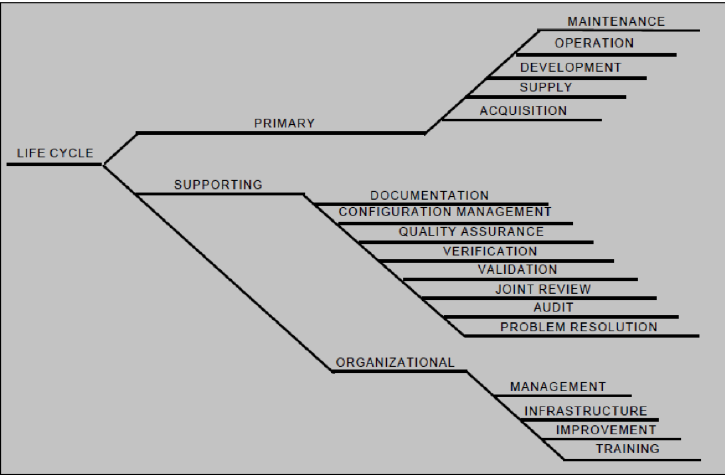
\includegraphics[scale=0.4]{res/images/ISO_12207.png}
	\caption{Processi del ciclo di vita del software, secondo lo standard ISO/IEC 25010:2011}
\end{figure}
Di tutti questi processi, elenchiamo quelli su cui ci siamo concentrati maggiormente.
\begin{itemize}
	\item Tra i \textit{processi primari}:
		\begin{itemize}
			\item \textbf{Sviluppo};
			\item \textbf{Fornitura}.
		\end{itemize}
	\item Tra i \textit{processi di supporto}:
		\begin{itemize}
			\item \textbf{Documentazione};
			\item \textbf{Gestione della configurazione};
			\item \textbf{Accertamento della qualità};
			\item \textbf{Verifica};
			\item \textbf{Validazione};
			\item \textbf{Risoluzione dei problemi}.
		\end{itemize}
	\item Tra i \textit{processi organizzativi}:
	\begin{itemize}
		\item \textbf{Gestione} (dei processi, comunicazione e rischi);
		\item \textbf{Infrastruttura}.
	\end{itemize}
\end{itemize}
\subsection{ISO/IEC 25010:2011}
In questo standard troviamo la parte di qualità del software, sostituisce l'ISO/IEC 9126 dal 2011 in poi.\\
In particolare aggiunge il modello della qualità in uso del software.\\
\begin{enumerate}
	\item \textbf{Efficacia:} precisione e completezza con cui gli utenti raggiungono i risultati desiderati.
	\item \textbf{Efficienza:} risorse spese in relazione agli obiettivi raggiunti (e in relazione all'efficacia).
	\item \textbf{Soddisfazione:} soddisfazione dell'utente, relativo ai suoi bisogni soddisfatti dal software.\\Solitamente la soddisfazione dipende dal soddisfacimento di \textit{utilità}, \textit{fiducia nel software}, \textit{gradimento} e \textit{comfort}.
	\item \textbf{Libertà da rischi:} grado con cui il software mitiga i possibili rischi.\\In particolare:
		\begin{itemize}
			\item mitigazione rischi economici;
			\item mitigazione rischi di salute e sicurezza;
			\item mitigazione rischi ambientali.
		\end{itemize}
	\item \textbf{Context coverage:} grado con cui il software può essere usato con efficacia\textsubscript{G}, efficienza\textsubscript{G}, soddisfazione e libertà da rischi, in qualunque contesto.
\end{enumerate}
Consultare la sezione ISO/IEC 9126 per altre informazioni sulla qualità del software.
\subsection{ISO/IEC 9126}
ISO/IEC 9126 è uno standard internazionale per valutare la qualità del software.\\
Questo standard fornisce un modello di qualità e 3 tipologie di metriche, queste 4 sezioni vengono riportate di seguito.\\
\begin{figure}[h!]
	\centering
	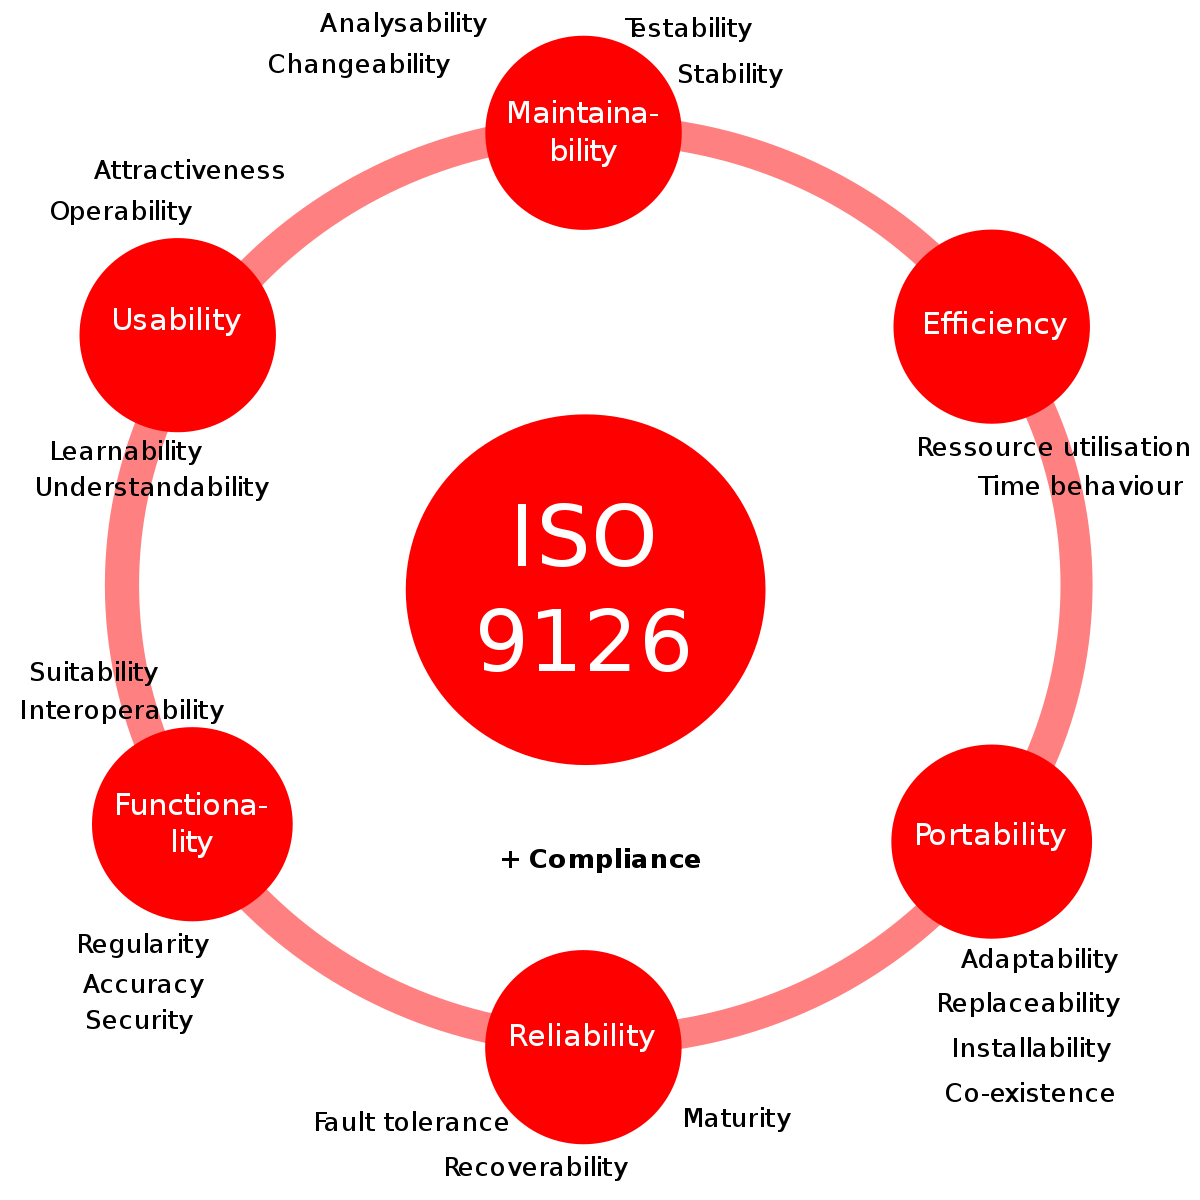
\includegraphics[scale=0.15]{res/images/ISO_9126.png}
	\caption{Figura esplicativa del modello della qualità software esterna ed interna dello standard ISO/IEC 9126}
\end{figure}
\subsubsection{Metriche per la qualità interna}
Definisce metriche applicabili al codice sorgente non eseguibile. Idealmente, la qualità interna determina la qualità esterna.\\
Viene rilevata tramite \textbf{analisi statica}.
\subsubsection{Metriche per la qualità esterna}
Definisce metriche applicabili al software in esecuzione che ne misurano i comportamenti tramite test. Idealmente, la qualità esterna determina la qualità in uso.\\
Viene rilevata tramite \textbf{analisi dinamica}.
\subsubsection{Metriche per la qualità in uso}
Definisce metriche applicabili solo quando il prodotto è finito e utilizzato in condizioni reali.
\subsubsection{Modello della qualità del software}
\begin{enumerate}
	\item \textbf{Funzionalità:} il software deve fornire funzioni che soddisfino i bisogni emersi nell'\textsc{Analisi dei Requisiti}.\\In particolare il software deve avere le seguenti caratteristiche:
		\begin{itemize}
			\item Appropriatezza;
			\item Accuratezza;
			\item Interoperabilità;
			\item Sicurezza.
		\end{itemize}
	\item \textbf{Affidabilità:} il software deve mantenere un certo livello di prestazioni quando utilizzato in condizione specificate.\\In particolare il software deve avere le seguenti caratteristiche:
		\begin{itemize}
			\item Maturità;
			\item Robustezza;
			\item Recuperabilità.
		\end{itemize}
	\item \textbf{Efficienza:} il software deve eseguire le proprie funzioni con minimo tempo e consumo di risorse possibile.\\In particolare efficienza\textsubscript{G} nel tempo, con veloci tempi di risposta e nello spazio, con una appropriata quantità di risorse.
	\item \textbf{Usabilità:} il software deve essere comprensibile e poter essere studiato senza troppe difficoltà.\\In particolare il software deve avere le seguenti caratteristiche:
		\begin{itemize}
			\item Comprensibilità;
			\item Apprendibilità;
			\item Operabilità;
			\item Attrattiva.
		\end{itemize}
	\item \textbf{Manutenibilità:} il software deve potersi evolvere con modifiche, correzioni e adattamenti.\\In particolare il software deve avere le seguenti caratteristiche:
		\begin{itemize}
			\item Analizzabilità;
			\item Modificabilità;
			\item Stabilità;
			\item Testabilità.
		\end{itemize}
	\item \textbf{Portabilità:} il software deve poter essere trasferito da un ambiente hardware/software ad un altro seguendo le evoluzioni tecnologiche.\\In particolare il software deve avere le seguenti caratteristiche:
		\begin{itemize}
			\item Adattabilità;
			\item Installabilità;
			\item Conformità;
			\item Sostituibilità.
		\end{itemize}
\end{enumerate}

	
\end{document}
